\documentclass[addpoints]{exam}
\usepackage[left=2.1cm,right=3.1cm,bottom=3cm,footskip=0.75cm,headsep=0.5cm]{geometry}
\usepackage[english]{babel}
\usepackage{amsmath,amssymb}
\usepackage{listings}
\usepackage{xcolor}
\usepackage{graphicx}
\definecolor{lightlightgray}{rgb}{0.95,0.95,0.95}
\definecolor{lila}{rgb}{0.8,0,0.8}
\definecolor{mygray}{rgb}{0.5,0.5,0.5}
\definecolor{mygreen}{rgb}{0,0.8,0.26}
%\lstdefinestyle{java} {language=java}
\lstset{language=R,
	basicstyle=\ttfamily,
	keywordstyle=\color{lila},
	commentstyle=\color{lightgray},
	stringstyle=\color{mygreen}\ttfamily,
	backgroundcolor=\color{white},
	showstringspaces=false,
	numbers=left,
	numbersep=10pt,
	numberstyle=\color{mygray}\ttfamily,
	identifierstyle=\color{blue},
	xleftmargin=.1\textwidth, 
	%xrightmargin=.1\textwidth,
	escapechar=§,
	%literate={\t}{{\ }}1
	breaklines=true,
	postbreak=\mbox{\space}
}
\usepackage[utf8]{inputenc}

\pointsinrightmargin
%\bracketedpoints
\boxedpoints

\title{\textbf{Trial Exam ADA WS 2021/22}}
\author{}
\date{}

% auskommentieren, wenn Antworten nicht angezeigt werden sollen
\printanswers

\begin{document}
	\maketitle
	
	\begin{questions}
		\section*{Part 1}
		\question[1] If Missing Values of INCOME depend on AGE, they are
		\begin{checkboxes}
			\choice Missing completly at Random
			\choice Not Missing at All
			\CorrectChoice Not Missing at Random
			\choice Missing at Random
		\end{checkboxes}
	
		\question[1] You want to test if men and woman have different income. What kind of test should yu use?
		\begin{checkboxes}
			\choice Z-score test
			\choice 1-tailed t-test
			\CorrectChoice 2-tailed t-test
			\choice F-test
		\end{checkboxes}
	
		\question[1] What does the Central Limit Theorem states?
		\begin{checkboxes}
			\CorrectChoice That the distribution of sample means approximates a normal distribution as the sample size get larger, regardless of the population's distribution.
			\choice That the distribution of the sample means approximates a normal distribution for only a sample size of $n<30$, regardless of the population's distribution.
			\choice That the distribution of sample means approximates a normal distribution as the sample size get larger, only if the population's distribution is a normal distribution.
			\choice That the distribution of the sample means approximates a normal distribution for only a sample size of $n=30$, regardless of the population's distribution.
		\end{checkboxes}
	
		\question[1] What statement of the Log transformation is correct?
		\begin{checkboxes}
			\choice The log transformation is used to prepare the data for further use. It replaces missing values with better guessed values.
			\choice The log transformation is only used to make left skewed distributions normally distributed. It allows to use powerful statistical procedures that only apply if the data is normally distributed.
			\choice The log transformation can be used to make not skewed distributions more skewed. It allows better interpretation of the data.
			\CorrectChoice The log transformation is used to make highly skewed distributions less skewed/normally distributed. It allows to use powerful statistical procedures that only apply if the data is normally distributed.
		\end{checkboxes}
	
		\question[1] You can handle missing values by deleting the subjects with mussing values.
		\begin{checkboxes}
			\choice TRUE, but only if the missing values are nominal scaled.
			\CorrectChoice TRUE, but if you can't fill the missing spots with sample means.
			\choice TRUE
			\choice FALSE
		\end{checkboxes}
	
		\question[1] Which statement about descriptive analysis is \textbf{wrong}?
		\begin{checkboxes}
			\choice Univariate analysis deals with only a single attribute and is mainly used for paramters of location and parameters of dispersion.
			\choice The interpretability of histograms is strongly dependent of the number of bins and the width of each interval.
			\CorrectChoice The frequency distribution can only be represented by a histogram.
			\choice Bi-variate analysis deals with the relationship between two varaibles and is mainly used for measurements of correlation.
		\end{checkboxes}
	
		\question[1] The attribute \textit{size} has the values "small", "medium", "large". What level of measurement is represented?
		\begin{checkboxes}
			\CorrectChoice \textit{Size} is based on an ordinal scale.
			\choice \textit{Size} is based on an nominal scale.
			\choice \textit{Size} is based on an interval scale.
			\choice \textit{Size} is based on an ratio scale.
		\end{checkboxes}
	
		\question[1] What is a hypothesis?
		\begin{checkboxes}
			\choice A research question the results will answer.
			\choice A statistical method for calculating the extend to which the results could have happend by chance.
			\choice A theory that underpins the study.
			\CorrectChoice A belief concering a parameter that the researcher wants to test through the data collected in a study.
		\end{checkboxes}
	
		\question[1] Multiple linear regression is used to:
		\begin{checkboxes}
			\choice Describe the relationship between one dependent variable and one independent variable.
			\CorrectChoice Describe the relationship between one dependent variable and multiple independent variables.
			\choice Describe the relationship between multiple dependent variables and one independent variable.
			\choice Describe the relationship between multiple dependent variables and multiple independent variables.
		\end{checkboxes}
	
		\question[1] The value for Model Sum of Squares (SSM) describes:
		\begin{checkboxes}
			\choice The distribution of the residuals.
			\CorrectChoice The total variance of the data.
			\choice The explained variance.
			\choice The unexplained variance.
		\end{checkboxes}
	
		\section*{Part 2}
		You found an old data set from 1981 online. Since you have always paid attention in the "Applied Data Analysis" excercise, it was no problem for you to import this data set into R under the variable name \textbf{data}. In this second part of the exam, we will mainly deal with this data set. The following table shows the first 5 lines of the 100-observation data set.
		\begin{center}
			\begin{tabular}{c|c|c|c|c|c|c}
				\textbf{gender} & \textbf{age} & \textbf{education} & \textbf{height} & \textbf{weight} & \textbf{IQ} & \textbf{ID} \\
				\hline
				0 & 34 & 1 & 189 & 99 & 100 & 1 \\
				1 & 56 & 2 & 156 & 54 & 110 & 2 \\
				0 & 21 & 3 & 173 & 67 & 107 & 3 \\
				2 & 45 & 2 & 178 & 71 & 122 & 4 \\
				1 & 32 & 2 & 171 & 69 & 98 & 5
			\end{tabular}
		\end{center}
	
		\question[1\half] To check the fit of a linear model, different values are determined. The following figure shows one step of a common procedure. Assign the labels to the illustration:
		\begin{center}
			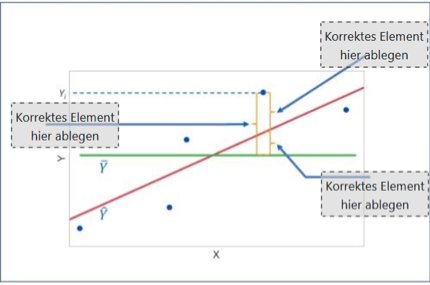
\includegraphics[scale=0.5]{errrorsplit.png}
		\end{center}
		\begin{itemize}
			\item Total error
			\item Residual
			\item Explained error
		\end{itemize} 
		\begin{solution}
			Total error = Residual + Explained error
		\end{solution}
	
		\question[3\half] We want to use another numeric variable to estimate the weight of a person. We choose the height and the age as possible candidates for the independent variable. Look at the two plots and decide which variable is more suitable as estimator for the weight. Explain you choice.
		\begin{center}
			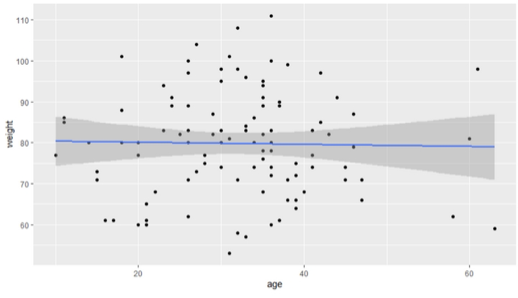
\includegraphics[scale=0.5]{plot1.png}
			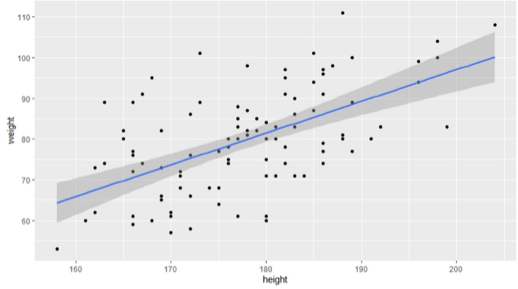
\includegraphics[scale=0.5]{plot2.png}
		\end{center}
		\begin{solution}
			Height is more suitable because slope $\neq 0$ $\Rightarrow$ correlation between height and weight
		\end{solution}
	
		\question[4] What is the purpose of R-squared? How is this value calculated abd what does is express? Describe the role played by the values "Total Sum of Squares" (SST), "Model Sum of Squares" (SSM) and "Error Sum of Squares" (SSE) in this context. Also name another measure to determine the quality of a linear model. 
		\begin{solution}
				\begin{align}
					R^2 = \frac{\text{Explained Error}}{\text{Total Error}} = \frac{SSM}{SST} \notag
				\end{align}
				Measure for goddness of fit, value of 1 indicates perfect fit, value of 0 indicates no fit at all. $R^2$ increase in multiple linear models with the number of parameters, better measures will also include the number of paramters like AIC.
		\end{solution}
	
		\question[7] Next we want to create linear models with R and assess some metrics to describe the fit between the models and the data. One model should use the height and the other should use the age as independet variable. Please create a short R-script to create the models and to output some metrics for these models.
		\begin{solution}
			\begin{lstlisting}
model1 = lm(weight ~ height, data = data)
model2 = lm(weight ~ age, data = data)

summary(model1)
summary(model2)
			\end{lstlisting}
		\end{solution}
	
		\question[4] For the two linear models to be created in R previously, R would give the following two outputs in the console.
		Which output belongs to which independent variable (height or age)? Evaluate the fit of the models using the metrics. Interpret R-squared in particular.
		\begin{center}
			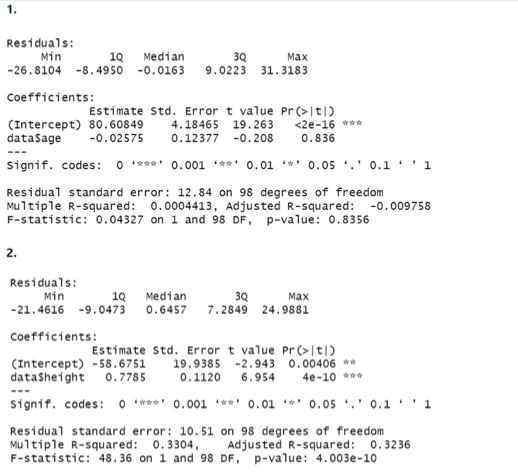
\includegraphics[scale=0.5]{r-output.png}
		\end{center}
		\begin{solution}
			output 1: weight $\sim$ age \\
			output 2: weight $\sim$ height, better $R^2$ (0.3304 vs. 0.0004413 for other model) $\Rightarrow$ loking at significance for parameters, age is not significant at all, height is significant ($\ast\ast\ast$ and p-value for height = 0 is $4\cdot 10^{-10}$)
		\end{solution}
	\end{questions}
\end{document}